% espacio entre parrafos
\setlength{\parskip}{5mm}
% sangria
\setlength{\parindent}{5mm}

\linespread{1.1}%
\selectfont	

\section{Introducción}

Los receptores de TV Digital, como los que funcionan de acuerdo al 
Sistema Argentino de Televisión Digital Terrestre (SATVD-T), deben contar con 
la  implementación de un \textit{zapper}.

Un \textit{zapper} es el componente de \textit{software} del decodificador mediante el
cual el usuario interactúa para sintonizar y ver canales. 
Permite además configurar el decodificador, administrar contenido multimedia 
y navegar la Guía de Programación Electrónica (EPG).

\emph{ZaMBA} (Zapper Multifunción Básico Argentino) es la implementación de
un \textit{zapper}, desarrollada por el laboratorio
LIFIA de la Universidad Nacional de La Plata. \emph{ZaMBA} está 
desarrollado en C++ y Lua; es Software Libre y la licencia utilizada es LGPLv2.

Entre las características implementadas por \textit{ZaMBA} se pueden destacar las siguientes:
\begin{itemize}
\item Escaneo de canales.
\item Cambio de canal.
\item Canales  favoritos y bloqueados.
\item Control de volúmen.
\item Configuración de salidas de audio y video.
\item Configuración de \textit{aspect ratio}.
\item Guía electrónica de programación.
\item Control parental.
\item Subtítulos.
\item Soporte de actualizaciones.
\item \textit{Middleware} de aplicaciones (\textit{Ginga.ar}).
\end{itemize}


Este documento presenta la arquitectura, herramientas y librerías necesarias para el desarrollo y extensión de ZaMBA.
Tambiíen se incluyen detalles sobre los principales módulos y clases que lo componen.
Luego se explica mediante diagramas de secuencia UML, cómo interactuan diferentes componentes de ZaMBA para ciertos casos de interés.
Finalmente, se explican las diferentes opciones de personalización existentes.


\section{Tecnologías y herramientas de desarrollo}
Para el desarrollo de ZaMBA se puede utilizar un entorno de desarrollo integrado (IDE), como Eclipse-CDT o Kdevelop, así también como trabajar 
desde un editor de texto y una terminal. Minimamente se requiere de un compilador C++, preferiblemente GCC a partir de la versión 4.6.3, un interprete de python 
(a partir de la versión 2.7.3), y CMake a partir de su versión 2.8. Con estas tres herramientas más las librerías externas requeridas (listadas más adelante), 
se tiene todo lo necesario para compilar el código fuente de ZaMBA.

Las librerías externas requeridas son las siguientes:
\begin{enumerate}
\item Componentes de Boost (a partir de la versión 1.46):
\begin{enumerate}
\item System
\item Filesystem (versión 3)
\item Thread
\item Date\_time
\item Math\_tr1
\end{enumerate}
\item BerkeleyDB
\item Lua51
\item Gtk2
\item LibVLC
\item XercesC (a partir de la versión 2.8)
\item LibEV
\item Zlib
\end{enumerate}

Para más información leer el documento build.pdf.

\section{Arquitectura de \emph{ZaMBA}}

Los módulos que componen la arquitectura de \emph{ZaMBA} se describen a  continuación:

\begin{itemize}
\item \textbf{util:}
implementa un conjunto muy variado de funciones, las cuales, son utilizadas por el resto de los módulos. 
Se pueden destacar: el manejo de \textit{buffers}, control de procesos, \textit{loop} de eventos, entre otras.

\item \textbf{canvas:}
implementa la funcionalidad que permite crear y controlar una interfaz gráfica. La funcionalidad incluye: manejo 
de ventanas, entrada de teclado, dibujado 2D, \textit{rendering} de video, etc. \\Dicha funcionalidad se implementa en diferentes
motores gráficos, lo que abstrae al usuario de esta librería de la implementación utilizada.

\item \textbf{mpegparser:}
permite demultiplexar las secciones de control y los flujos de datos obtenidos en un \textit{Transport Stream}, a partir del uso de filtros y notificar la ocurrencia de las mismas.\\
Provee la funcionalidad necesaria para obtener las secciones de control PAT, PMT, NIT, entre otras y los flujos de audio, video y datos.  

\item \textbf{zapper:}
provee funcionalidad para la sintonización y reproducción de \emph{Canales}. Permite configurar multiples características como por ejemplo: control de volúmen, salidas de video,
\textit{aspect ratio}, clasificación parental, canales favoritos.

\item \textbf{luaz:}
exporta los módulos necesarios para poder utilizar la funcionalidad de la librería \emph{zapper} desde un \textit{script} Lua.
\end{itemize}

En las próximas secciones los módulos descriptos son detallados. La figura \ref{zamba:modules} presenta la organización de los mismos.

\begin{figure}[ht!]
\centering
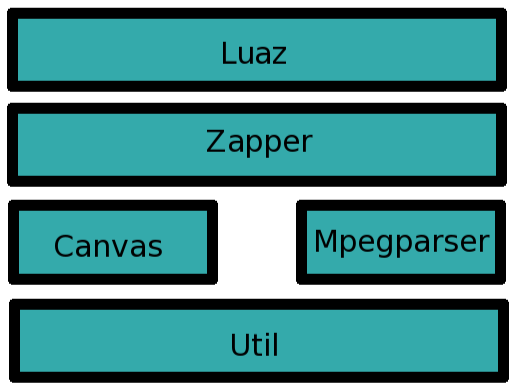
\includegraphics[scale=0.50]{../resources/zamba-modules}
\caption{Arquitectura de \emph{ZaMBA}}
\label{zamba:modules}
\end{figure}

\section{Diagramas de secuencia}

\subsection{Ejecución de aplicación interactiva}
En el siguiente diagrama de secuencia se puede ver como se instancia el \textit{middleware Ginga.ar} cuando se ha descargado una aplicación NCL. 
Para esto interactuan objetos de las librerías \textit{zapper} y \textit{mpegparser}. 
El diagrama se inicia cuando un objeto \texttt{dtv-zapper::ApplicationController} recibe una notificación de que se descargó la aplicación.
\begin{figure}[ht!]
\centering
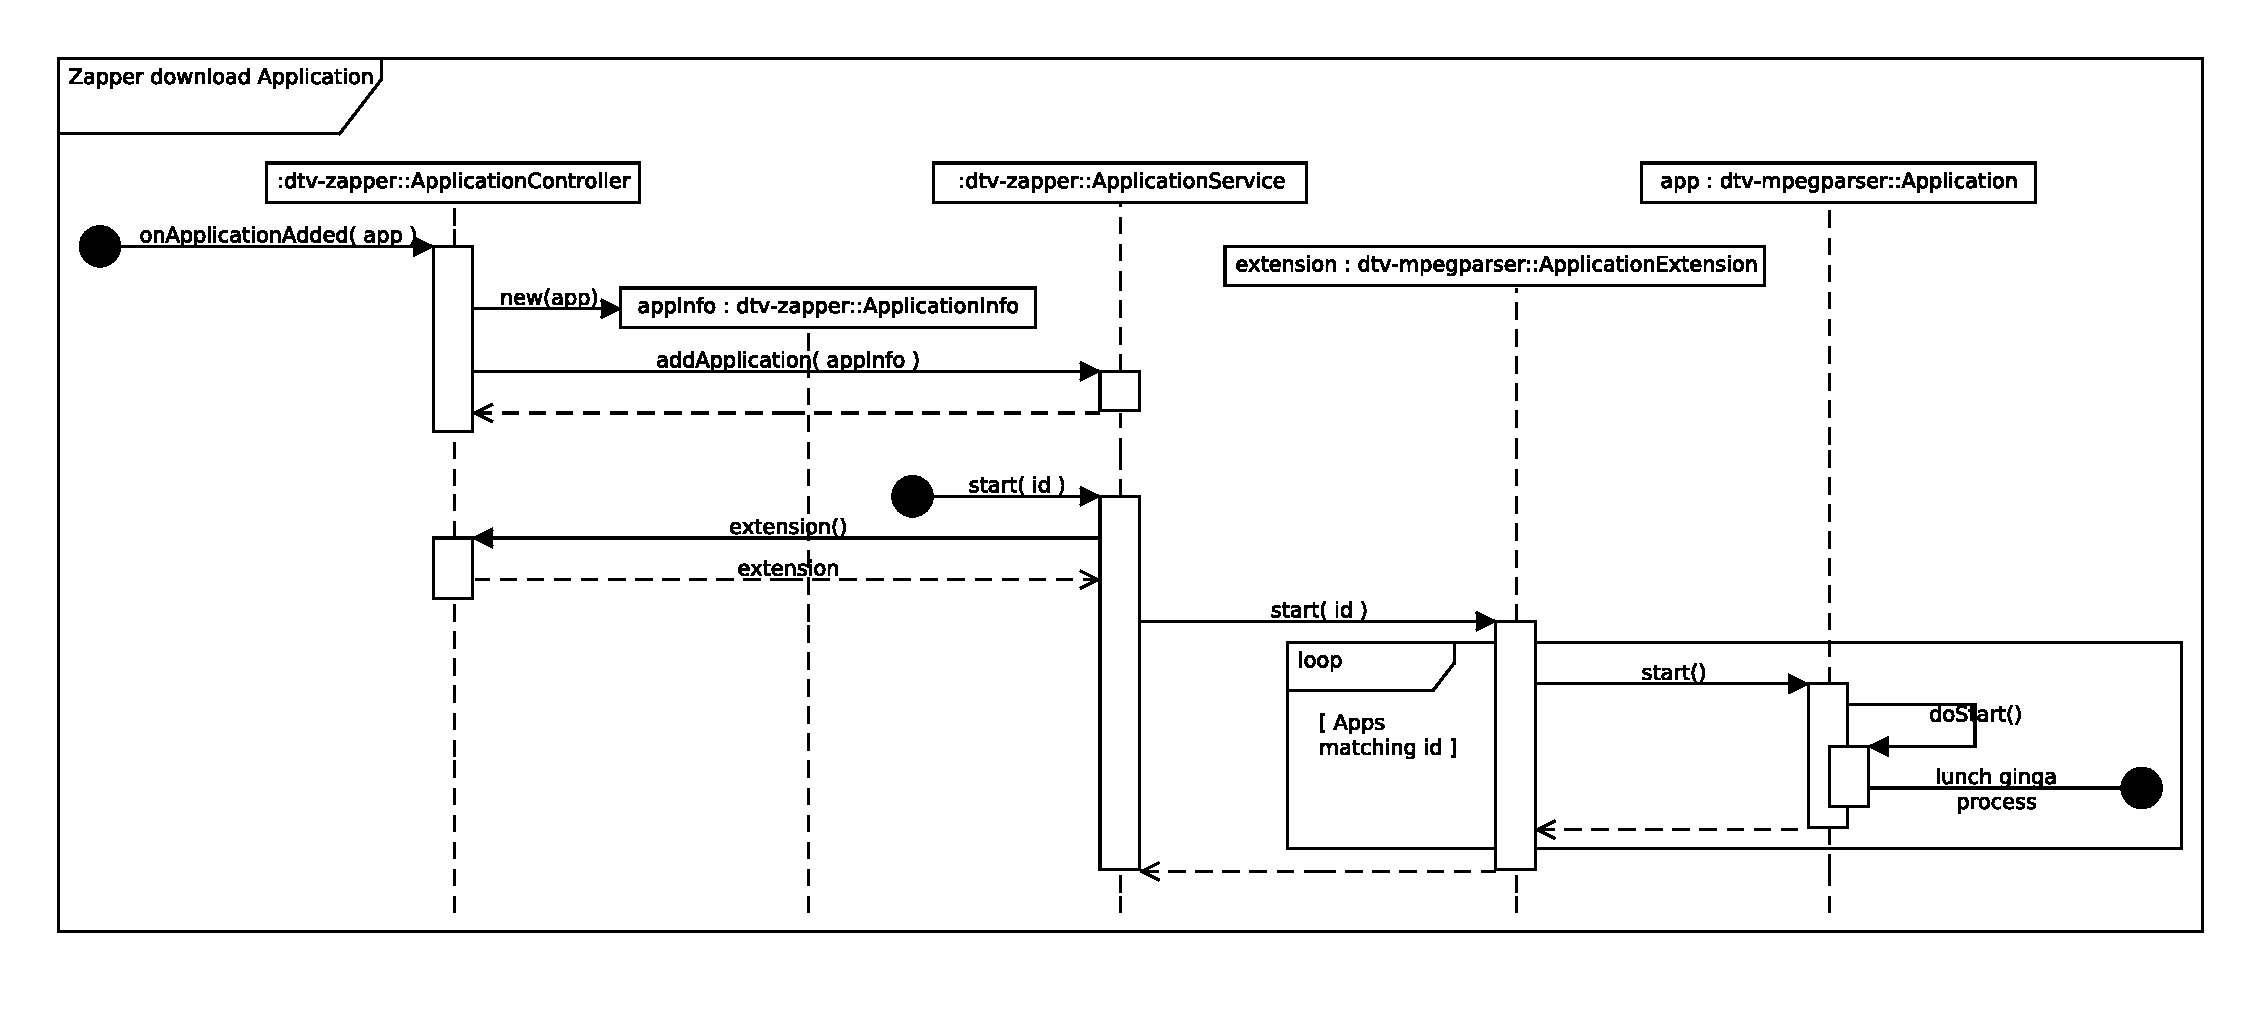
\includegraphics[scale=0.35,angle=-90]{../resources/uml-sequence-diagram-zapper-start-ginga}
\end{figure}

\pagebreak 
\subsection{Cambio de canal}
En el siguiente diagrama de secuencia se puede ver como se realiza un cambio de canal. Comienza cuando al objeto \texttt{dtv-zapper::ChannelPlayer}
le llega una solicitud para cambiar de canal. Este interactúa con objetos de la librería \textit{zapper} para actualizar la reproducción y determinar si el 
canal solicitado está o no bloqueado.
\begin{figure}[ht!]
\centering
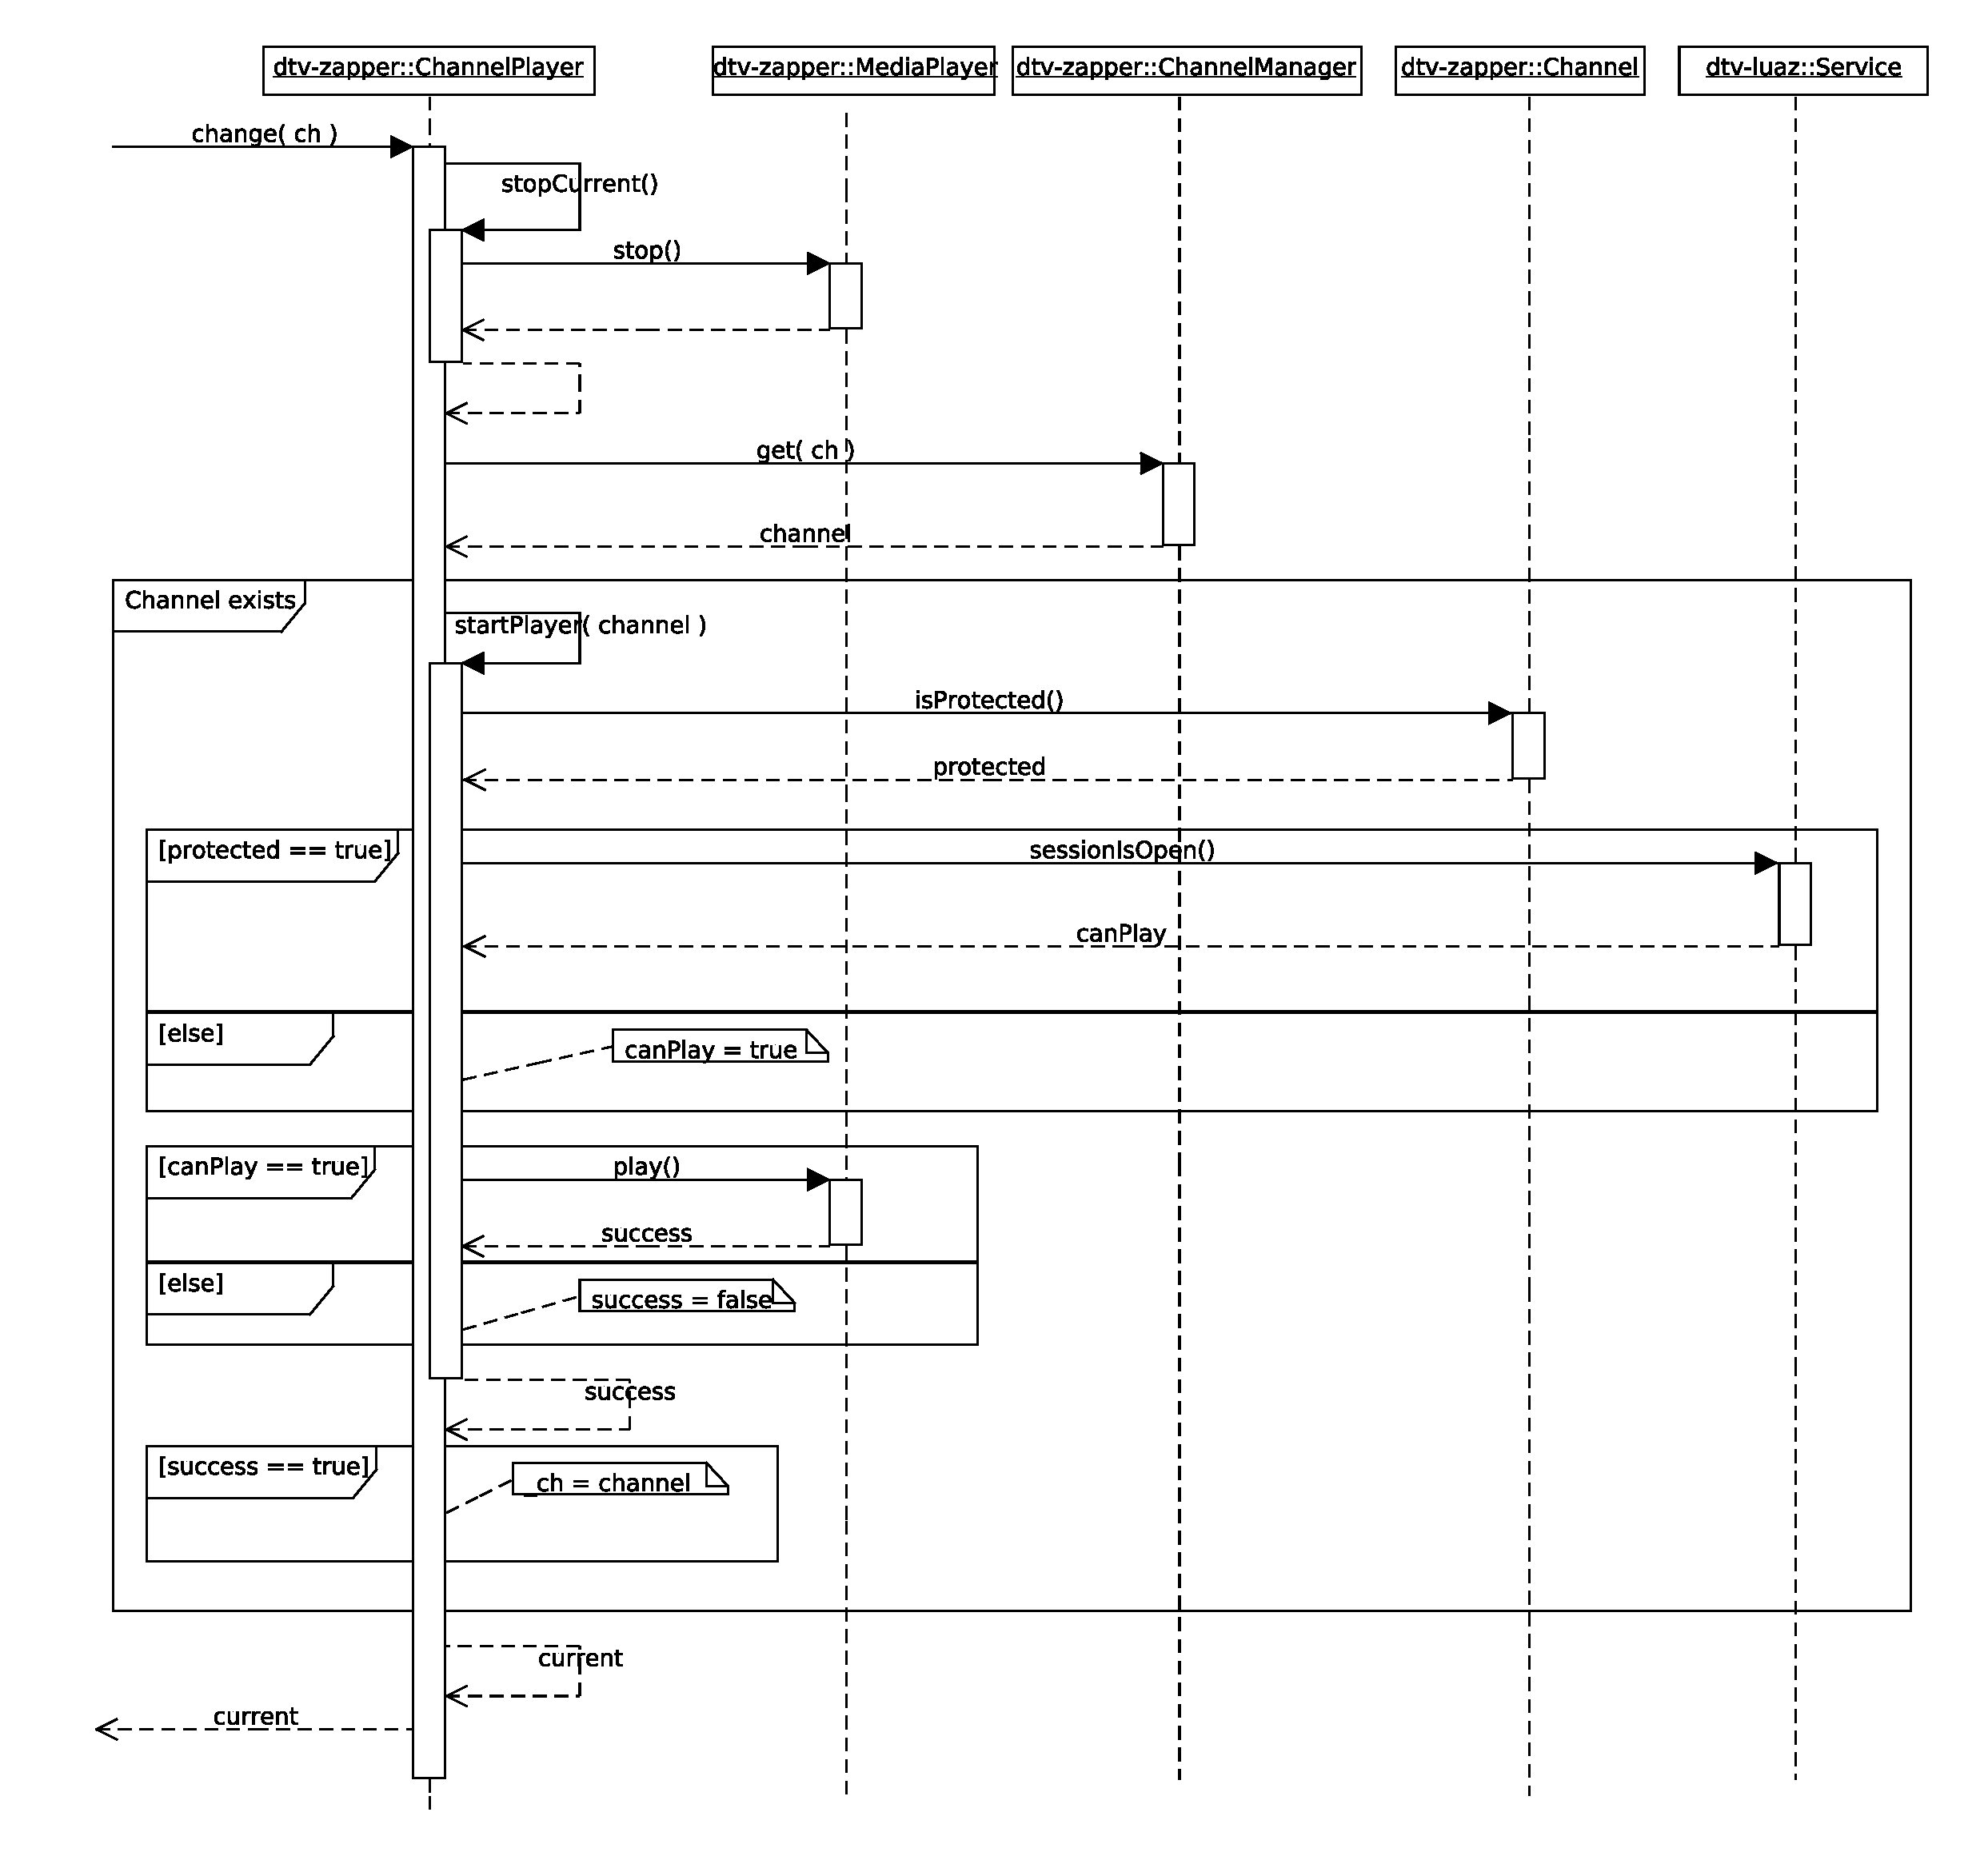
\includegraphics[scale=0.40]{../resources/uml-sequence-diagram-zapper-change-channel}
\end{figure}

\section{Personalización}
\emph{ZaMBA} permite la personalización de los colores así como también de la imagen que se utilizará con el logo.

\subsection{Colores}
Los widgets tienen una paleta de colores que indica como deberán dibujarse. Esto permite definir diferentes colores para el fondo, los bordes o cualquier otra componente.

En \texttt{colors.lua} se definen colores mediante su composición rgb, junto con las paletas que son usadas en la mayoría de los widgets. 
También se definen otras paletas para los widgets que no usan los esquemas de colores definidos anteriormente, esto se hace en los archivos donde se haga uso de los respectivos widgets.
\pagebreak
\begin{lstlisting}[
	language=xml,
	title=Ejemplo de tablas de colores,
	keywordstyle=\color{blue},
	commentstyle=\color{gray},
	stringstyle=\color{red},
	tabsize=4,
	showstringspaces=false,
	columns=fullflexible,
	breaklines=true,
	frame=none]
	
menuColorTable = {
		bgColor = Color.Black,
		selectedColor = Color.White
}

comboboxColorTable = {
	bgColor = Color.Blue,
	bgLabelColor = Color.None
}
\end{lstlisting}

\subsection{Logo e icono}
Para modificar la imagen con el logo de \emph{ZaMBA} se deberá reemplazar el archivo \texttt{Logo.png} que se encuentra dentro de los recursos de \emph{ZaMBA} por otra imagen. Y si se desea reemplazar el icono se deberá sobreescribir \texttt{icon.png}. 
Se deberá tener en cuenta que se deben respetar las dimensiones de las imágenes originales.

\section{Aplicaciones ZaMBA}

Las aplicaciones \emph{ZaMBA} son scripts que extienden la funcionalidad de \emph{ZaMBA}. Dichos scripts están escritos en el lenguaje de programación lua y deben tener obligatoriamente extensión \texttt{zmb}.

\subsection{Tipos de aplicaciones}
Las aplicaciones pueden ser de dos tipos, interactivas o servicios. Las primeras son aplicaciones que interactúan directamente con el usuario, la característica principal de éste tipo de aplicaciones es que tienen el control sobre los eventos de teclado, si una tecla es presionada durante la ejecución de una aplicación interactiva, es ésta quien decide como tratarla. Las únicas teclas que no pueden ser manejadas por la aplicación son \texttt{escape} y \texttt{exit}, las mismas sirven para cerrar la aplicación y devolver el control a \emph{ZaMBA}. Otra característica importante de las aplicaciones interactivas es que pueden dibujar en pantalla, para ésto debe hacer uso de la librería \texttt{canvas}. Un juego es un ejemplo típico de aplicación interactiva.\\
Las aplicaciones de tipo servicio son aplicaciones que se ejecutan en background, lo que significa que no dibujan en pantalla y no interactúan directamente con el usuario, son notificadas con los mismos eventos que las aplicaciones interactivas, pero el flujo normal de \emph{ZaMBA} no se verá alterado. Al recibir las notificaciones de los eventos, los servicios pueden conocer información sobre el uso de \emph{ZaMBA} y las acciones que el usuario lleva a cabo. Un ejemplo típico es un servicio que mantiene e informa estadísticas sobre los canales que son vistos por el usuario.

\subsection{Implementacíón de aplicaciones}

Una aplicación debe definir una función llamada \texttt{describe}, el propósito de ésta es proporcionar información sobre la aplicación; para ello la función debe retornar una tabla con los siguientes campos:

\begin{itemize}
	\item name: String que representa el nombre de la aplicación, este nombre será mostrado en la lista de selección de aplicaciones.
	\item interactive: Booleano que determina si la aplicación es interactiva o no.
	\item methods: Tabla que debe contener las siguientes entradas:
	\begin{itemize}
		\item start: Función que es llamada al ejecutar una aplicación. Si la aplicación es interactiva se pasará como parámetro un objeto superficie donde la aplicación podrá dibujar. Éste campo es obligatorio.
		\item stop: Función que es llamada al detener la ejecución de la aplicación. Debe ser utilizada para la finalizaci\'on de la aplicación y liberación de recursos.  Éste campo es obligatorio.
		\item startSetup: Función que es llamada cuando una aplicación debe ser configurada (ver Configuración de una aplicación), el método recibe un objeto \texttt{surface} donde debe dibujar su interfaz de configuración. Este campo es opcional y solo debe ser definido si se desea realizar alguna configuración sobre la aplicaci\'on.
		\item stopSetup: Función que es llamada cuando una aplicación sale de la ventana de configuración. No es obligatorio que sea implementada.
		\item handleEvent: Función que es llamada cada vez que se produce un evento. Los eventos son tablas con dos campos, \texttt{type} y \texttt{value}, el campo \texttt{type} determina el tipo del evento mientras que el campo \texttt{value} toma un valor cuya semántica depende de \texttt{type}. Los tipos de eventos son:
		\begin{itemize}
			\item Key: Se produce con un evento de teclado, el campo \texttt{type} es igual a 'key' mientras que en \texttt{value} se almacena el \texttt{keycode} de la tecla presionada. Además este evento define un campo extra llamado \texttt{isUp} cuyo valor es un boleano que representa si la tecla fue presionada o soltada.
			\item Timer: Se produce cuando un \texttt{timer} ha expirado (ver módulo \texttt{timer}). El campo \texttt{type} es igual a 'timeOut' y el campo \texttt{value} del evento posee el identificador del timer que lo ha producido.
			\item Cambio de canal: Se produce cuando se cambia un canal, el campo \texttt{type} es igual a \mbox{'channelChanged'} mientras que en \texttt{value} se almacena el id del canal sintonizado.
		\end{itemize}
		El campo  \texttt{handleEvent} es opcional.
	\end{itemize}
\end{itemize}


Adicionalmente la tabla puede definir los siguientes campos de forma opcional:
\begin{itemize}
	\item desc: String que contiene la descripción de la aplicación
	\item version: String que contiene la versión de la aplicación
\end{itemize}

\subsection{Módulo timer}

El módulo \texttt{timer} no es más que una tabla que contiene dos funciones, \texttt{timer.register} y \texttt{timer.cancel}, la primera permite registrar un timer y la segunda cancelarlo. Cuando se registra un timer comienza a correr un reloj, si éste llega al tiempo indicado, sin ser cancelado, se le enviar\'a un evento de tipo 'timeOut' a la aplicaci\'on.
El prototipo de la función \texttt{timer.register} es:\\
\texttt{timer.register( milliseconds )}\\
donde \texttt{milliseconds} es el tiempo (en milisegundos) que transcurrir\'an hasta que se despache el evento a la aplicaci\'on. La función tiene como valor de retorno al identificador del timer, el cual es un valor único y sirve para identificar al timer vencido al momento de manejar el evento.
El prototipo de la función \texttt{timer.cancel} es:\\
\texttt{timer.cancel( timerID )}\\
dónde el parámetro \texttt{timerID} identifica al timer a cancelar.

\subsection{Configuración de una aplicación}

Cada aplicaci\'on deber\'a implementar su propia configuraci\'on. Al m\'etodo \texttt{startSetup} se le pasa una \texttt{surface}, en la cual se deber\'a dibujar la informaci\'on necesaria. Mediante el manejo de eventos se puede implementar la interacci\'on con el usuario. Una vez presionada la tecla \texttt{escape} o \texttt{exit} se cerrar\'a la configuración y la aplicación recibirá el callback \texttt{stopSetup}.

\subsection{Restricciones y consideraciones}

Las aplicaciones interactivas pueden utilizar la API de canvas para crear nuevas \texttt{surfaces}, las mismas se utilizan como una \texttt{surface} regular excepto por el hecho de que no pueden utilizar el método \texttt{autoFlush}, ésto implica que ninguna \texttt{surface} será dibujada en pantalla hasta que ésta sea compuesta en la \texttt{surface} principal. La \texttt{surface} principal es enviada como parámetro al método \texttt{start} una vez que la aplicación es iniciada.

Las aplicaciones tienen acceso tanto a las librerías lua del sistema como a las librerías propias de \emph{ZaMBA} por lo cual el programador de aplicaciones debe tener especial cuidado durante su uso. El mal uso de éstas librerías puede derivar en un incorrecto funcionamiento de \emph{ZaMBA}. Cualquier error producido en una aplicación causará que la misma sea terminada inmediatamente, lo que producirá la llamada a el método stop de la aplicación. Cuando un error se haya producido el log pertinente será mostrado en consola.

